\documentclass[
a4paper,                        % paper size
11pt,                           % font size
twoside,                        % two sided
footsepline,                    % add a line to separate the footer
headsepline,                    % add a line to separate the header
headexclude,                    % header does not belong to the text
footexclude,                    % footer does not belong to the text
pagesize,                       % set the pagesize in a DVI document
bibtotocnumbered,               % add the bibliography to the TOC
idxtotoc                        % add the index to the TOC
%openright,                      % start a new chapter on the right page
%,DIV12
%,draft
]{scrreprt}

\usepackage{nameref}            % nameref, varioref, hyperref must be
                                % used in this order (see hyperref
                                % README)!
\usepackage[draft]{varioref}    % defines \vref
\usepackage{hyperref}           % automatically creates links when
                                % using pdflatex, defines \url
\usepackage{ifpdf}              % defines \ifpdf
\usepackage{graphicx}           % handles graphics
\usepackage{makeidx}            % creates the index
\usepackage{fancybox}

%%%%%%%%%%%%%%%%%%%%%%%%%%%%%%%%%%%%%%%%%%%%%%%%%%
%%%%%%%%%%%%%%%%%%%%%%%%%%%%%%%%%%%%%%%%%%%%%%%%%%
%%%%%%%%% New Commands and Environments %%%%%%%%%%
%%%%%%%%%%%%%%%%%%%%%%%%%%%%%%%%%%%%%%%%%%%%%%%%%%
%%%%%%%%%%%%%%%%%%%%%%%%%%%%%%%%%%%%%%%%%%%%%%%%%%
\newcommand{\es}{\textsf{ESPResSo}}
\newcommand{\ie}{\textit{i.e.\/}}
\newcommand{\eg}{\textit{e.g.\/}}
\newcommand{\etal}{\textit{et al.\/}}

\newcommand{\variant}[2]{(#1) \texttt{#2}\\}
%\newcommand{\lit}[1]{\texttt{#1}}
\newcommand{\var}[1]{\textrm{\textit{#1}}}
\newenvironment{syntax}{%
  \begin{Sbox}
    \begin{minipage}{0.9\linewidth}
    }{%
    \end{minipage}
  \end{Sbox}
  \begin{center}
    \fbox{\TheSbox}
  \end{center}
}

%%%%%%%%%%%%%%%%%%%%%%%%%%%%%%%%%%%%%%%%%%%%%%%%%%
%%%%%%%%%%%%%%%%%%%%%%%%%%%%%%%%%%%%%%%%%%%%%%%%%%
%%%%%%%%%%%%%%%% Other Settings %%%%%%%%%%%%%%%%%%
%%%%%%%%%%%%%%%%%%%%%%%%%%%%%%%%%%%%%%%%%%%%%%%%%%
%%%%%%%%%%%%%%%%%%%%%%%%%%%%%%%%%%%%%%%%%%%%%%%%%%
\pagestyle{headings}
\makeindex

%%%%%%%%%%%%%%%%%%%%%%%%%%%%%%%%%%%%%%%%%%%%%%%%%%
%%%%%%%%%%%%%%%%%%%%%%%%%%%%%%%%%%%%%%%%%%%%%%%%%%
%%%%%%%%%%%%%%%%% Main Document %%%%%%%%%%%%%%%%%%
%%%%%%%%%%%%%%%%%%%%%%%%%%%%%%%%%%%%%%%%%%%%%%%%%%
%%%%%%%%%%%%%%%%%%%%%%%%%%%%%%%%%%%%%%%%%%%%%%%%%%
\begin{document}
\titlehead{
  \begin{center}
    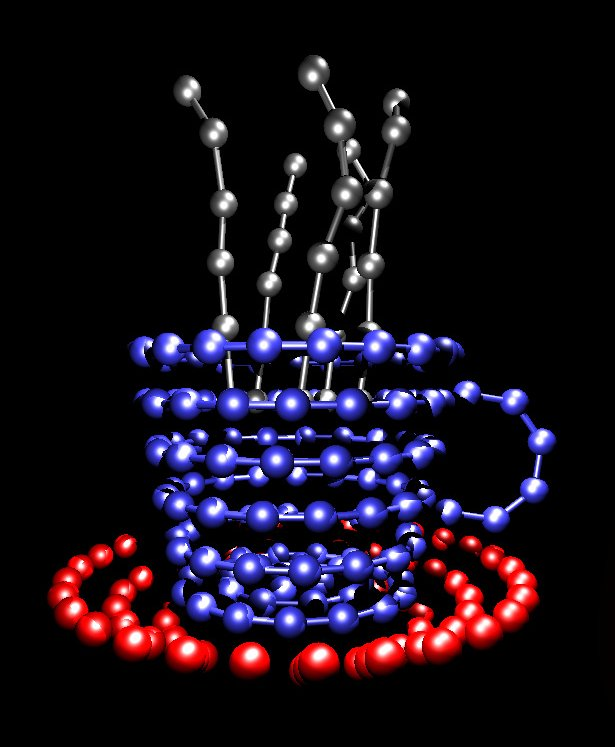
\includegraphics[width=5cm]{logo.jpg}
  \end{center}
}
%\subject{}
\title{\es{} User's Guide}
%\author{}
%\date{\today}
\maketitle

\tableofcontents

\chapter{Introduction}
\label{chap:intro}

(new)

\begin{itemize}
\item \es{} is a generic soft matter simulation packages
\item for molecular dynamics simulations in soft matter research
\item focussed on coarse-grained models
\item employs modern algorithms (Lattice-Boltzmann, DPD, P3M, \ldots)
\item written in C for maximal portability
\item Tcl-controlled
\item parallelized
\end{itemize}

\section{Guiding principles}
\label{sec:ideas}

(from paper: 2.1 Goals and principles)

\es
\begin{itemize}
\item does \emph{not} do the physics for you!
\item requires you to understand what you do (can not be used as a
  black box)
\item gives you maximal freedom (flexibility)
\item is extensible
\item integrates system setup, simulation and analysis, as this can't
  be strictly separated in soft matter simulations
\item has no predefined units
\item sets as few defaults as possible
\end{itemize}

\section{Algorithms contained in \es}

The following algorithms are implemented in \es{}:

\begin{itemize}
\item ensembles: NVE, NVT, NpT
\item charged systems:
  \begin{itemize}
  \item P3M for fully periodic systems
  \item ELC and MMM-family of algorithms for charged systems with
    non-periodic boundary conditions
  \item Maggs algorithm 
  \end{itemize}
\item Hydrodynamics:
  \begin{itemize}
  \item DPD (as a thermostat)
  \item Lattice-Boltzmann
  \end{itemize}
\end{itemize}

\section{Basic program structure}
\label{sec:structure}

(from paper: 2.2 Basic program structure)

\begin{itemize}
\item Control level: \texttt{Tcl}
\item ``Kernel'' written in \texttt{C}
\item This user's guide will focus on the control level
\end{itemize}

\section{On units}
\label{sec:units}
\index{units}
\index{length unit}
\index{time unit}
\index{energy unit}
\index{physical units}

What is probably one of the most confusing subjects for beginners of
\es is, that \es does not predefine any units.  While most MD programs
specify a set of units, like, for example, that all lengths are
measured in \AA ngstr\"om or nanometers, times are measured in nano- or
picoseconds and energies are measured in $\frac{kJ}{\mathrm{mol}}$,
\es does not do so.

Instead, the length-, time- and energy scales can be freely chosen by
the user.  A length of $1.0$ can mean a nanometer, an \AA ngstr\"om,
or a kilometer - depending on the physical system, that the user has
in mind when he writes his \es-script.  The user can choose the unit
system that suits the system best.

When creating particles that are intended to represent a specific type
of atoms, one will probably use a length scale of \AA ngstr\"om.  This
would mean, that \eg the parameter $\sigma$ of the Lennard-Jones
interaction between two atoms would be set to twice the van-der-Waals
radius of the atom in \AA ngstr\"om.  Alternatively, one could set
$\sigma$ to $2.0$ and measure all lengths in multiples of the
van-der-Waals radius.

The second choice to be made is the energy (and time-) scale.  One can
for example choose to set the Lennard-Jones parameter $\epsilon$ to
the energy in $\frac{kJ}{\mathrm{mol}}$.  Then all energies will be
measured in that unit.  Alternatively, one can choose to set it to
$1.0$ and measure everything in multiples of the van-der-Waals binding
energy.

As long as one remains within the same unit system throughout the
whole \es-script, there should be no problems.

\section{Requirements}
\label{sec:requirements}
\index{requirements}

The following libraries and tools are required to be able to compile
and use \es:

\begin{description}
\item[Tcl/Tk] \index{Tcl/Tk} \es{} requires the Toolkit Command
  Language Tcl/Tk \footnote{\url{http://www.tcl.tk/}} in the version
  8.3 or later.  Some example scripts will only work with Tcl 8.4. You
  do not only need the interpreter, but also the header files and
  libraries.  Depending on the operating system, these may come in
  separate development packages. If you want to use a graphical user
  interface (GUI) for your simulation scripts, you will also need Tk.
  
\item[FFTW] \index{FFTW} In addition, \es{} needs the FFTW library
  \footnote{\url{http://www.fftw.org/}} for Fourier transforms.
  ESPResSo can work with both the 2.1.x and 3.0.x series. Again, the
  header files are required.
  
\item[MPI] \index{MPI} Finally, if you want to use \es{} in parallel,
  you need a working MPI environment (version 1.2). Currently, the
  following MPI implementations are supported:
  \begin{itemize}
  \item LAM/MPI is the preferred variant
  \item MPICH, which seems to be considerably slower than LAM/MPI in
    our benchmarks.
  \item On AIX systems, \es{} can also use the native POE parallel
    environment.
  \item On DEC/Compaq/HP OSF/Tru64, \es{} can also use the native
    dmpirun MPI environment.
  \end{itemize}
\end{description}


\section{Syntax description}
\label{sec:syntax}


Throughout the user's guide, formal definitions of the syntax of
several Tcl-commands can be found. The following conventions are used
in these decriptions:
\begin{itemize}
\item Different \emph{variants} of a command are labelled \variant{1},
  \variant{2}, \ldots
\item Keywords and literals of the command that have to be typed
  exactly as given are written in \lit{typewriter} font.
\item If the command has variable arguments, they are set in
  \var{italic font}. The description following the syntax definition
  should contain a detailed explanation of the argument and its
  type.
\item \texttt{\alt{\var{alt1} \asep \var{alt2}}} specifies, that one
  of the alternatives \var{alt1} or \var{alt2} can be used.
\item \texttt{\opt{\var{argument}}} specifies, that the arugment
  \var{argument} is optional, \ie{} it can be omitted.
\item When an optional argument or a whole command is marked by a
  superscript label (\fmark{1}), this denotes that the argument can
  only be used, when the corresponding feature (see appendix
  \vref{chap:features}) specified in ``Required features'' is
  activated.
\end{itemize}


\minisec{Example}

\renewcommand{\variant}[1]{\par\rawvariant{#1}}
\begin{essyntaxbox}
  \variant{1} 
  constraint wall normal \var{n_x} \var{n_y} \var{n_z} 
  dist \var{d} type \var{id}
  
  \variant{2}
  constraint sphere center \var{c_x} \var{c_y} \var{c_z} 
  radius \var{rad} direction \var{direction} type \var{id} 
  
  \require{1}{%
    \variant{3}
    constraint rod center \var{c_x} \var{c_y} 
    lambda \var{lambda}
  } 
  
  \require{2,3}{%
    \variant{4}
    constraint ext_magn_field \var{f_x} \var{f_y} \var{f_z} 
  }

  \begin{features}
    \required{CONSTRAINTS}
    \required[1]{ELECTROSTATICS}
    \required[2]{ROTATION}
    \required[3]{DIPOLES}
  \end{features}

\end{essyntaxbox}
\renewcommand{\variant}[1]{\rawvariant{#1}}

%%% Local Variables: 
%%% mode: latex
%%% TeX-master: "ug"
%%% End: 

\chapter{Tutorial}
\label{chap:tutorial}

\section{Quick installation}

\index{configure}\index{make}

If you have the requirements (see section \vref{sec:requirements})
installed, in many cases, to compile \es{}, it is enough to execute
the following sequence of two steps in the directory where you have
unpacked the sources:
\begin{verbatim}
> configure
> make
\end{verbatim}

In some cases, \eg{} when \es{} needs to be compiled for several
different platforms or when different versions with different sets of
features are required, it might be useful to execute the commands not
in the source directory itself, but to start \texttt{configure} from
another directory (see section \vref{sec:builddir}). Furthermore, many
features of \es{} can be selectively turned on or off in the local
configuration header of \es{} (see section \vref{sec:myconfig}) before
starting the compilation with \texttt{make}.

The shell script \texttt{configure} prepares the source code for
compilation. It will determine how to use and where to find the
different libraries and tools required by the compilation process, and
it will test what compiler flags are to be used.  The script will find
out most of these things automatically.  If something is missing, it
will complain and give hints how to solve the problem.  The
configuration process can be controlled with the help of a number of
options that are explained in section \vref{sec:configure}.

The command \texttt{make} will compile the source code. Depending on
the options passed to the program, \texttt{make} can also be used for
a number of other things:
\begin{itemize}
\item It can install and uninstall the program to some other
  directories. However, normally it is not necessary to actually
  \textit{install} \es{} to run it.
\item It can test the \es{} program for correctness.
\item It can build the documentation.
\end{itemize}
The details of the usage of \texttt{make} are described in section
\vref{sec:make}.

When these steps have successfully completed, \es{} can be started
with the command (see section \vref{sec:run})
\begin{verbatim}
> Espresso
\end{verbatim}

\section{Running \es{}}
\begin{itemize}
\item interactive use (sample session)
\item small sample session
\item script execution
\end{itemize}


\section{Doing a simulation}

\begin{itemize}
\item \verb!erice_tutorial! or appendix A from paper
\item Reference to \verb!tutorial.tcl! (?)
\end{itemize}


%%% Local Variables: 
%%% mode: latex
%%% TeX-master: "ug"
%%% End: 

% Copyright (C) 2010,2011,2012,2013 The ESPResSo project
% Copyright (C) 2002,2003,2004,2005,2006,2007,2008,2009,2010 
%   Max-Planck-Institute for Polymer Research, Theory Group
%  
% This file is part of ESPResSo.
%   
% ESPResSo is free software: you can redistribute it and/or modify it
% under the terms of the GNU General Public License as published by the
% Free Software Foundation, either version 3 of the License, or (at your
% option) any later version.
%  
% ESPResSo is distributed in the hope that it will be useful, but
% WITHOUT ANY WARRANTY; without even the implied warranty of
% MERCHANTABILITY or FITNESS FOR A PARTICULAR PURPOSE.  See the GNU
% General Public License for more details.
%  
% You should have received a copy of the GNU General Public License
% along with this program.  If not, see <http://www.gnu.org/licenses/>.
%
\chapter{Getting, compiling and running \es}
\label{chap:install}
\index{Installation|textbf}

This chapter will describe how to get, compile and run the \es
software.  

\es releases are available as source code packages from the \es home
page\footnote{\url{http://espressomd.org}}.  This is where new users
should get the code.  The code within release packages is tested and
known to run on a number of platforms.  Alternatively, people that
want to use the newest features of \es or that want to start
contributing to the software can instead obtain the current
development code via the version control system software
\textsf{git}\footnote{\url{http://git.org}} from \es's project page at
the Savannah GNU server
\footnote{\url{https://savannah.nongnu.org/projects/espressomd/}}.
This code might be not as well tested and documented as the release
code; it is recommended to use this code only if you have already
gained some experience in using \es.

Unlike most other software, no binary distributions of \es are
available, and the software is usually not installed globally for all
users.  Instead, users of \es should compile the software themselves.
\index{features} The reason for this is that it is possible to
activate and deactivate various features before compiling the code.
Some of these features are not compatible with each other, and some of
the features have a profound impact on the performance of the code.
Therefore it is not possible to build a single binary that can satisfy
all needs.  A user should always activate only those features that are
actually needed.  This means, however, that learning how to compile
\es is a necessary evil.  The build system of \es uses the GNU
autotools, which are developed since more than 20 years and allow to
compile software easily on a wide range of platforms.

\section{Running \texttt{configure}}
\label{sec:configure}
\index{configure}

\todo[inline]{Description of basic options: \keyword{CPPFLAGS},
  \keyword{CFLAGS}, \keyword{LDFLAGS}}

The first step of building \es is to run the shell script
\codebox{configure} which is to be found in the top level source
directory.  The script collects all the information required by the
compilation process.  It will determine how to use and where to find
the compiler, as well as the different libraries and tools required by
the compilation process, and it will test what compiler flags are to
be used.  The script will find out about most of these things
automatically.  If something is missing, it will complain and give
hints how to solve the problem.  The generic syntax of calling the
\codebox{configure} script is:
\begin{code}
configure [\var{options} ...] [\var{variable}=\var{value} ...]
\end{code}

If you are using the development source code from the \textsf{git}
repository, before you can call \codebox{configure}, it is necessary
to have the GNU autotools (\textsf{autoconf} and \textsf{automake})
installed. Then you can call the script \codebox{bootstrap.sh} from
the top level source directory, which will generate the
\codebox{configure} script.

\subsection{Source and build directories}
\label{ssec:builddir}
\index{build directory} \index{source directory}

Usually, when a program is compiled, the resulting binary files are
put into the same directory as the sources of the program.  In \es's
build system, the \emph{source directory} that contains all the source
files is completely separated from the \emph{build directory}, where
the files created by the build process are put.  The location of the
build directory is the current working directory at the time when
\codebox{configure} is called.  In this way, you can build several
variants of \es, each variant having different activated features, and
for as many platforms as you want.  All further commands concerning
compiling and running \es have to be called from the build directory.

\paragraph{Example}
When the source directory is \codebox{\$srcdir} (\ie the files where
unpacked to this directory), then the build directory can be set to
\codebox{\$builddir} by calling the \codebox{configure}-script from
there:
\begin{code}
cd $builddir
$srcdir/configure
make
Espresso
\end{code}

\subsection{Options}
\label{ssec:configureoptions}

\index{configure options} The behaviour of \codebox{configure} can be
controlled by the means of command line options.  In the following
only those command line options that are specific to \es will be
explained.  For a complete list of options and explanations thereof,
call
\begin{code}
configure --help
\end{code}

\begin{description}
\item[\texttt{--with-myconfig=MYCONFIG\_HEADER}] This option sets the
  name of the local configuration header (see \vref{sec:myconfig}). It
  defaults to ``\texttt{myconfig.h}''.
\item[\texttt{--with-mpi=\alt{\lit{yes} \asep \lit{no} \asep
      \lit{guess}}}/ \texttt{--without-mpi}] By default,
  \codebox{configure} will automatically determine whether an MPI
  compiler is available.  If it is, it will use it.  If you specify
  \codebox{--without-mpi} or \codebox{--with-mpi=no}, then MPI will
  not be used, even if it is available.
\item[\texttt{--with-efence} / \texttt{--without-efence}] Whether or
  not to use the ``electric fence'' memory debugging library.
  \footnote{\url{http://freshmeat.net/projects/efence/}} Efence is not
  used by default.
\item[\texttt{--with-tcl=TCL}] By default, \texttt{configure} will
  automatically determine which version of Tcl is used.  If the wrong
  version is chosen automatically, you can specify the name of the
  library with this option, \eg \texttt{tcl8.4}.
\item[\texttt{--with-tk=TK} / \texttt{--without-tk}] By default, the
  GUI toolkit Tk is not used by \es. This option can be used to
  activate Tk and to specify which Tk version to use, \eg{}
  \texttt{tk8.4}. If you only specify \texttt{--with-tk} and do not
  give a version number, \texttt{configure} will try to automatically
  deduce the right version.
\item[\texttt{--with-fftw} / \texttt{--without-fftw}] This can
  be used to specify whether the FFTW library is to be used, and which
  version.  By default, version 3 will be used if it is found,
  otherwise version 2 is used.  Note that quite a number of central
  features of \es require FFTW.
\item[\texttt{--with-cuda=path} / \texttt{--without-cuda}] This switch
  enables CUDA support. \texttt{path} should be the path to the CUDA
  directory, which can be omitted if it is the NVIDIA default path,
  \ie \texttt{/usr/local/cuda}. The variable \texttt{NVCCFLAGS} can
  be used to define compiler flags for the NVIDIA CUDA-compiler
  \texttt{nvcc}. For example, \texttt{NVCCFLAGS = "{}-gencode
    arch=compute_20,code=sm_20"{}} will compile code only for Fermi
  cards.  Default is to compile for compute models 1.1 and 2.0,
  i.e. everything with a G90 chip or newer.  Note that we require at
  least compute model 1.1.
\end{description}

\section{\texttt{make}: Compiling,  testing and installing \es}
\label{sec:make}

The command \texttt{make} is mainly used to compile the \es source
code, but it can do a number of other things. The generic syntax of
the \texttt{make} command is:
\begin{code}
make [\var{options}] [\var{target}...] [\var{variable}=\var{value}]
\end{code}
When no target is given, the target \texttt{all} is used. The
following targets are available:
\begin{description}
\item[\texttt{all}] Compiles the complete \es source code. The
  variable \lit{myconf} can be used to specify the name of the
  configuration header to be used.
\item[\texttt{check}] Runs the testsuite. By default, all available
  tests will be run on 1, 2, 3, 4, 6, or 8 processors. Which tests are
  run can be controlled by means of the variable \texttt{tests}, which
  processor numbers are to be used can be controlled via the variable
  \texttt{processors}. Note that depending on your MPI installation,
  MPI jobs can only be run in the queueing system, so that \es{} will
  not run from the command line. In that case, you may not be able to
  run the testsuite, or you have to directly submit the testsuite script
  \verb!testsuite/test.sh! to the queueing system.\\
  \textbf{Example:} \verb!make check tests="madelung.tcl" processors="1 2"!\\
  will run the test \texttt{madlung.tcl} on one and two processors.
\item[\texttt{clean}] Deletes all files that were created during the
  compilation.
\item[\texttt{mostlyclean}] Deletes most files that were created
  during the compilation. Will keep for example the built doxygen
  documentation and the \es{} binary.
\item[\texttt{dist}] Creates a \texttt{.tar.gz}-file of the \es{}
  sources.  This will include all source files as they currently are
  in the source directory, \ie{} it will include local changes.  This
  is useful to give your version of \es{} to other people.
  The variable \texttt{extra} can be used to specify additional
  files and directories that are to be included in the archive
  file. \\
  \textbf{Example:} \verb!make dist extra="myconfig.h internal"!\\
  will create the archive file and include the file
  \texttt{myconfig.h} and the directory \texttt{internal} with all
  files and subdirectories.
\item[\texttt{install}] Install \es. The variables \texttt{prefix} and
  \texttt{exec-prefix} can be used to specify the installation
  directories, otherwise the defaults defined by the
  \texttt{configure} script are used. \texttt{prefix} sets the prefix
  where all \es files are to be installed, \texttt{exec-prefix} sets
  the prefix where the executable files are to be installed and is
  required only when there is an architecture-specific directory.\\
  \textbf{Example:} \verb!make install prefix=/usr/local!\\
  will install all files below \texttt{/usr/local}.
\item[\texttt{uninstall}] Uninstalls \es, \ie removes all files that
  were installed during \texttt{make install}. The variables are
  identical to the variables of the \texttt{install}-target.
\item[\texttt{ug\ \ }] Creates the User guide in the \texttt{doc/ug}
  subdirectory (only when using the development sources).
\item[\texttt{dg\ \ }] Creates the Developers' guide in the
  \texttt{doc/dg} subdirectory (only when using the development
  sources).
\item[\texttt{doxygen\ \ }] Creates the Doxygen code documentation in the
  \texttt{doc/doxygen} subdirectory.
\item[\texttt{tutorials\ \ }] Creates the \es tutorials in the
  \texttt{doc/tutorials} subdirectory.
\item[\texttt{doc\ }] Creates all documentation in the \texttt{doc}
  subdirectory (only when using the development sources).
\end{description}

A number of options are available when calling \texttt{make}.  The
most interesting option is probably \texttt{-j \textit{num\_jobs}},
which can be used for parallel compilation on computers that have more
than one CPU or core.  \textit{num\_jobs} specifies the maximal number
of jobs that will be run.  Setting \textit{num\_jobs} to the number of
available processors speeds up the compilation process significantly.

\section{Running \es}
\label{sec:run}

When \es is found in your path, it can be run via
\begin{code}
Espresso [\var{tcl\_script} [\var{args}]]
\end{code}

\index{interactive mode} When \es{} is called without any arguments,
it is started in the interactive mode, where new commands can be
entered on the command line. When the name of a \textit{tcl\_script}
is given, the script is executed. \textit{N\_processors} is the number
of processors that are to be used. Any further arguments are passed to
the script. Note that depending on your MPI installation, MPI jobs can
only be run in the queueing system, so that \es will not run from
the command line.


\section{\texttt{myconfig.h}: Activating and deactivating features}
\label{sec:myconfig}

\index{features} \index{myconfig.h} \index{configuration header} \es
has a large number of features that can be compiled into the binary.
However, it is not recommended to actually compile in all possible
features, as this will slow down \es significantly.  Instead, compile
in only the features that are actually required.  A strong gain in
speed can be achieved, by disabling all non-bonded interactions except
for a single one, e.g. \feature{LENNARD_JONES}.  For the developers,
it is also possible to turn on or off a number of debugging messages.
The features and debug messages can be controlled via a configuration
header file that contains C-preprocessor declarations. Appendix
\vref{chap:features} lists and describes all available features.  When
no configuration header is provided by the user, a default header,
found in src/myconfig-default.h, will be used that turns on the
default features.  The file \texttt{myconfig-sample.h} in the source
directory contains a list of all possible features that can be copied
into your own configuration file.

When you distinguish between the build and the source directory, the
configuration header can be put in either of these. Note, however,
that when a configuration header is found in both directories, the one
in the build directory will be used.

By default, the configuration header is called \texttt{myconfig.h}.
The name of the configuration header can be changed either when the
\texttt{configure}-script is called with the option
\mbox{\texttt{--with-myconfig}} (see section \vref{sec:configure}), or
when \texttt{make} is called with the setting
\mbox{\texttt{myconfig=}\textit{myconfig\_header}} (see section
\vref{sec:make}).

The configuration header can be used to compile different binary
versions of \es with a different set of features from the same source
directory.  Suppose that you have a source directory \texttt{\$srcdir}
and two build directories \texttt{\$builddir1} and
\texttt{\$builddir2} that contain different configuration headers:

\begin{itemize}
\item \texttt{\$builddir1/myconfig.h}:
\begin{code}
#define ELECTROSTATICS
#define LENNARD-JONES
\end{code}

\item \texttt{\$builddir2/myconfig.h}:
\begin{code}
#define LJCOS
\end{code}
\end{itemize}

\noindent Then you can simply compile two different versions of \es via
\begin{code}
cd $builddir1
$srcdir/configure
make

cd $builddir2
$srcdir/configure
make
\end{code}


%%% Local Variables: 
%%% mode: latex
%%% TeX-master: "ug"
%%% End: 

\chapter{\es{} command reference}
\label{chap:ref}

(most from paper and from related pages)

\begin{itemize}
\item Will contain description of all Tcl-commands
\item Reference to appendix \vref{chap:quickref}
\item basic identifiers:
  \begin{itemize}
  \item particle type
  \item bonded interaction type
  \item molecule id
  \end{itemize}
\end{itemize}


\section{\texttt{inter}: Setting up interactions}
\label{sec:inter}
\begin{syntax}
  \variant{1}
  {inter 
    \var{part\_type\_id1} 
    \var{part\_type\_id2}
    \var{inter\_type} 
    [ \var{parameters}\ldots ]
  }
  \variant{2}
  {inter 
    \var{bond\_type\_id} \var{bond\_type} [
    \var{parameters}\ldots ]
  }
  \variant{3}
  {inter}
\end{syntax}
    % \section{Creating particles}
% \label{sec:part}
% \texttt{part}

% \section{Interactions}
% \label{sec:inter}
% \texttt{inter}

% \section{Analysis}
% \label{sec:analysis}

%%% Local Variables: 
%%% mode: latex
%%% TeX-master: "ug"
%%% End: 

% Copyright (C) 2010,2012,2013,2014,2015,2016 The ESPResSo project
% Copyright (C) 2002,2003,2004,2005,2006,2007,2008,2009,2010 
%   Max-Planck-Institute for Polymer Research, Theory Group
%  
% This file is part of ESPResSo.
%   
% ESPResSo is free software: you can redistribute it and/or modify it
% under the terms of the GNU General Public License as published by the
% Free Software Foundation, either version 3 of the License, or (at your
% option) any later version.
%  
% ESPResSo is distributed in the hope that it will be useful, but
% WITHOUT ANY WARRANTY; without even the implied warranty of
% MERCHANTABILITY or FITNESS FOR A PARTICULAR PURPOSE.  See the GNU
% General Public License for more details.
%  
% You should have received a copy of the GNU General Public License
% along with this program.  If not, see <http://www.gnu.org/licenses/>.
%
\chapter{Under the hood}
\label{chap:underhood}

\begin{itemize}
\item Implementation issues that are interesting for the user
\item Main loop in pseudo code (for comparison)
\end{itemize}

\section{Internal particle organization}
\label{sec:internal-particle-organization}

Since basically all major parts of the main MD integration have to
access the particle data, efficient access to the particle data is
crucial for a fast MD code. Therefore the particle data needs some
more elaborate organisation, which will be presented here. A particle
itself is represented by a structure (Particle) consisting of several
substructures (e. g. ParticlePosition, ParticleForce or
ParticleProperties), which in turn represent basic physical properties
such as position, force or charge. The particles are organised in one
or more particle lists on each node, called Cell cells. The cells are
arranged by several possible systems, the cellsystems as described
above. A cell system defines a way the particles are stored in \es{},
i. e. how they are distributed onto the processor nodes and how they
are organised on each of them. Moreover a cell system also defines
procedures to efficiently calculate the force, energy and pressure for
the short ranged interactions, since these can be heavily optimised
depending on the cell system. For example, the domain decomposition
cellsystem allows an order N interactions evaluation.

Technically, a cell is organised as a dynamically growing array, not
as a list. This ensures that the data of all particles in a cell is
stored contiguously in the memory. The particle data is accessed
transparently through a set of methods common to all cell systems,
which allocate the cells, add new particles, retrieve particle
information and are responsible for communicating the particle data
between the nodes. Therefore most portions of the code can access the
particle data safely without direct knowledge of the currently used
cell system. Only the force, energy and pressure loops are implemented
separately for each cell model as explained above.

The domain decomposition or link cell algorithm is implemented in
\es{} such that the cells equal the \es{} cells, i. e. each cell is a
separate particle list. For an example let us assume that the
simulation box has size $20\times 20\times 20$ and that we assign 2
processors to the simulation. Then each processor is responsible for
the particles inside a $10\times 20\times 20$ box. If the maximal
interaction range is 1.2, the minimal possible cell size is 1.25 for 8
cells along the first coordinate, allowing for a small skin of 0.05.
If one chooses only 6 boxes in the first coordinate, the skin depth
increases to 0.467. In this example we assume that the number of cells
in the first coordinate was chosen to be 6 and that the cells are
cubic. \es{} would then organise the cells on each node in a $6\times
12\times 12$ cell grid embedded at the centre of a $8\times 14 \times
14$ grid. The additional cells around the cells containing the
particles represent the ghost shell in which the information of the
ghost particles from the neighbouring nodes is stored. Therefore the
particle information stored on each node resides in 1568 particle
lists of which 864 cells contain particles assigned to the node, the
rest contain information of particles from other nodes.a

Classically, the link cell algorithm is implemented differently.
Instead of having separate particle lists for each cell, there is only
one particle list per node, and a the cells actually only contain
pointers into this particle list. This has the advantage that when
particles are moved from one cell to another on the same processor,
only the pointers have to be updated, which is much less data (4 rsp.
8 bytes) than the full particle structure (around 192 bytes, depending
on the features compiled in). The data storage scheme of \es{} however
requires to always move the full particle data. Nevertheless, from our
experience, the second approach is 2-3 times faster than the classical
one.

To understand this, one has to know a little bit about the
architecture of modern computers. Most modern processors have a clock
frequency above 1GHz and are able to execute nearly one instruction
per clock tick. In contrast to this, the memory runs at a clock speed
around 200MHz. Modern double data rate (DDR) RAM transfers up to
3.2GB/s at this clock speed (at each edge of the clock signal 8 bytes
are transferred). But in addition to the data transfer speed, DDR RAM
has some latency for fetching the data, which can be up to 50ns in the
worst case. Memory is organised internally in pages or rows of
typically 8KB size. The full $2\times 200$ MHz data rate can only be
achieved if the access is within the same memory page (page hit),
otherwise some latency has to be added (page miss). The actual latency
depends on some other aspects of the memory organisation which will
not be discussed here, but the penalty is at least 10ns, resulting in
an effective memory transfer rate of only 800MB/s. To remedy this,
modern processors have a small amount of low latency memory directly
attached to the processor, the cache.

The processor cache is organised in different levels. The level 1 (L1)
cache is built directly into the processor core, has no latency and
delivers the data immediately on demand, but has only a small size of
around 128KB. This is important since modern processors can issue
several simple operations such as additions simultaneously. The L2
cache is larger, typically around 1MB, but is located outside the
processor core and delivers data at the processor clock rate or some
fraction of it.

In a typical implementation of the link cell scheme the order of the
particles is fairly random, determined e. g. by the order in which the
particles are set up or have been communicated across the processor
boundaries. The force loop therefore accesses the particle array in
arbitrary order, resulting in a lot of unfavourable page misses. In
the memory organisation of \es{}, the particles are accessed in a
virtually linear order. Because the force calculation goes through the
cells in a linear fashion, all accesses to a single cell occur close
in time, for the force calculation of the cell itself as well as for
its neighbours. Using the domain decomposition cell scheme, two cell
layers have to be kept in the processor cache. For 10000 particles and
a typical cell grid size of 20, these two cell layers consume roughly
200 KBytes, which nearly fits into the L2 cache. Therefore every cell
has to be read from the main memory only once per force calculation.



%%% Local Variables: 
%%% mode: latex
%%% TeX-master: "ug"
%%% End: 

% Copyright (C) 2010 The ESPResSo project
% Copyright (C) 2002,2003,2004,2005,2006,2007,2008,2009,2010 Max-Planck-Institute for Polymer Research, Theory Group, PO Box 3148, 55021 Mainz, Germany
%  
% This file is part of ESPResSo.
%   
% ESPResSo is free software: you can redistribute it and/or modify it
% under the terms of the GNU General Public License as published by the
% Free Software Foundation, either version 3 of the License, or (at your
% option) any later version.
%  
% ESPResSo is distributed in the hope that it will be useful, but
% WITHOUT ANY WARRANTY; without even the implied warranty of
% MERCHANTABILITY or FITNESS FOR A PARTICULAR PURPOSE.  See the GNU
% General Public License for more details.
%  
% You should have received a copy of the GNU General Public License
% along with this program.  If not, see <http://www.gnu.org/licenses/>.
%
\chapter{Getting involved}
\label{chap:devel}

Up to date information about the development of \es
can be found at the web page \url{http://espressomd.org}
As the important information can change in time, we will not describe
its contents in detail but rather request the reader to
go directly to the URL.
Among other things, one can find information about the following topics there:

\begin{itemize}
\item FAQ
\item Latest stable release of \es and older releases
\item Obtaining development version of \es
\item Archives of both developers' and users' mailing lists
\item Registering to \es mailing lists
\item Submitting a bug report
\end{itemize}

\section{Community support and mailing lists}

If you have any questions concerning \es which you cannot
resolve by yourself, you may post a message to
the mailing list. Instructions on how to register to the mailing
lists and post messages can be found on the homepage 
\url{http://espressomd.org}.
Before posting a question and waiting for someone to answer, 
it may be useful to search the mailing list archives or FAQ and 
see if you can get the answer immediately.
For several reasons it is recommended to send all questions 
to the mailing lists rather than to contact individual developers:
\begin{itemize}
  \item All registered users get your message and you have a higher 
  probability that it is answered soon.
  \item Your question and the answers are archived and the archives
  can be searched by others.
  \item The answer may be useful also to other registered users.
  \item There may not be a unique answer to your problem and it may 
  be useful to get suggestions from different people.
\end{itemize}

Please remember that this is a community mailing list. It is other
users and developers who are answering your questions. They do it
in their free time and are not paid for doing it.


\section{Contributing your own code}

If you are planning to make an extension to \es or 
already have a piece of your own code which could be useful 
to others, you are very welcome to contribute it to 
the community. 
Before you start making any changes to the code, you
should obtain the current development version of it.
For more information about how to obtain the
development version, refer to the homepage \url{http://espressomd.org}.

It is also generally a good idea to contact the mailing lists before
you start major coding projects. It might be that someone else is
already working on the problem or has a solution at hand.

\section{Developers' guide}
\label{sec:dg}

Besides the User guide, \es also contains a Developers' guide which is
a programmer documentation automatically built from comments in the
source code and using Doxygen.  It provides a cross-referenced
documentation of all functions and data structures available in \es
source code. It can be built by typing
\begin{code}
  make dg
\end{code}
in the build directory. Afterwards it can be found
in the subdirectory of the build directory: \texttt{doc/dg/html/index.html}.

A recent version of this guide can also be found on the \es{} homepage
\url{http://espressomd.org}.

\section{User's guide}

If, while reading this user guide, you notice any mistakes or badly
(if at all) described features or commands, you are very welcome to
contribute to the guide and have others benefit from your knowledge.

For this, you should also checkout the development version as
described on the homepage. As the user guide, like all \es{} code, is
always in flow and changes are made regularly, there are already many
paragraphs marked with a ``todo'' box. To turn on these boxes, edit
the main file \texttt{doc/ug/ug.tex} and adapt the inclusion of the
\LaTeX{} package \texttt{todonotes}.

You can then build the user guide by typing
\begin{code}
  make ug
\end{code}



%%% Local Variables: 
%%% mode: latex
%%% TeX-master: "ug"
%%% End: 


\appendix
\chapter{\es{} quick reference}
\label{chap:quickref}

\begin{itemize}
\item Short reference table of all commands
\item Complete syntax of \es{} commands
\item Features required for different commands
\end{itemize}

\chapter{The MMM family of algorithms}
\label{chap:mmm}

\chapter{Maggs algorithm}
\label{chap:maggs}

\printindex

\end{document}


%%% Local Variables: 
%%% mode: latex
%%% TeX-master: t
%%% End: 
